\chapter{\IfLanguageName{dutch}{Stand van zaken}{State of the art}}
\label{ch:stand-van-zaken}

In het vorig hoofdstuk werd deze bachelorproef al kort ingeleid. In dit hoofdstuk zal de huidige kennis uit dit onderzoeksdomein verder besproken worden.

In sectie \ref{sec:chatbots} zal er besproken worden wat chatbots zijn, welke soorten er bestaan, wat de voor-en nadelen zijn, wat de verbeterpunten en toekomstmogelijkheden zijn en hoe chatbots er voor staan op het vlak van beveiliging hoe dit verbeterd kan worden.

In sectie \ref{sec:nlp} wordt er ingezoomd op Natural Language Processing en de subdomeinen NLU en NLG.

In sectie \ref{sec:nlp-platformen} zullen de interessantste platformen kort geïntroduceerd worden en zullen ze vergeleken worden met elkaar op basis van een aantal basiscriteria. Binnen dit onderzoek worden geen volledig betalende/enterprise NLP-platformen vergeleken/toegelicht.

\newpage
\section{Chatbots}
\label{sec:chatbots}

\subsection{Soorten}
\label{subsec:soorten}

\subsubsection{Rule-based chatbot}
\label{subsubsec:chatbots-soorten-rule-based-chatbot}

Dit is de eenvoudigste en het traagste type chatbot. Deze bot bevat geen machine learning of artificiële intelligentie, maar werkt op basis van voorgeprogrammeerde regels. Bij dit type kan je enkel communiceren via een vaste selectie vragen/bevelen en kan je bij antwoord van de chatbot ook enkel terug antwoorden door uit een lijst te kiezen. Dit type zorgt voor weinig vrijheid, waardoor het ook enkel goed is voor basis klantvragen. Doordat alles manueel geprogrammeerd moet worden, is het ook telkens veel werk om nieuwe regels toe te voegen en de functionaliteit uit te breiden. Indien je een bericht stuurt naar deze bot die hij niet kent, dan weet hij ook gewoonweg niet wat hij ermee moet doen. Het voordeel van dit type is dan wel dat hij altijd accuraat antwoordt geeft, net doordat alles voorgedefinieerd is. Binnen deze bachelorproef zullen chatbots van dit type niet onderzocht en verder toegelicht worden.

\begin{figure}[!htbp]
    \label{fig:rule-based-chatbot-example}
    \centering
    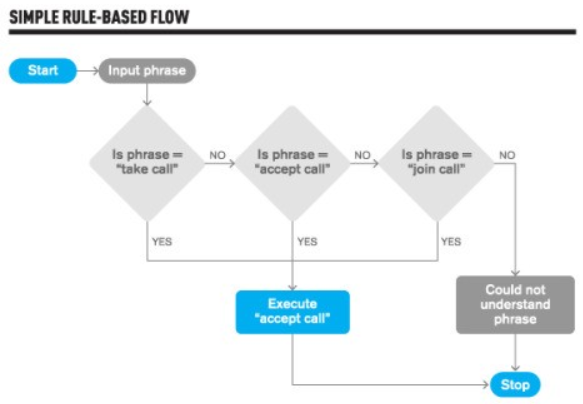
\includegraphics[width=0.8\textwidth]{rule-based-chatbot-example}
    \caption{Eenvoudige Flowchart van een rule-based chatbot \autocite{Shridhar2017}}
\end{figure}

\subsubsection{ML-based chatbot}
\label{subsubsec:chatbots-soorten-ml-based-chatbot}


Dit type chatbot wordt ook wel de NLP-chatbot of de AI-powered chatbot genoemd. Bij deze soort wordt in tegenstelling tot de rule-based chatbot wel sterk gebruik gemaakt van artificiële intelligentie en machine learning. De bot kan vragen beantwoorden die hij nog nooit eerder heeft gehoord en elimineert dus de limitatie van het rule-based type. NLP-chatbots leren van voorgaande taken en gaan op die manier zichzelf slimmer maken en hun kennis uitbreiden. Ze gebruiken ook speciale functies en algoritmes om de zinnen echt te verstaan en verder te verwerken. Dit type biedt de gebruiker veel meer vrijheid, maar is moeilijker om te ontwikkelen. De accuraatheid van deze soort is dan ook gemiddeld lager. Binnen deze bachelorproef zal de focus enkel liggen op chatbots van dit type. Wanneer er gesproken wordt over chatbots of gewoonweg bots, wordt er steeds een chatbot van dit type bedoeld.

\subsection{Voor-en nadelen}
\label{subsec:chatbots-voor-en-nadelen}

\subsubsection{Voordelen}
\label{subsubsec:chatbots-voor-en-nadelen-voordelen}

\begin{itemize}
    \item \textbf{Menselijke taken overnemen:} \\
    
    Chatbots worden ingezet voor heel wat verschillende toepassingen en kunnen menselijke taken overnemen. Een voorbeeld hiervan is reminders sturen van de agenda van een persoon zodat hij zelf niet meer hoeft te kijken. Chatbots nemen ook veel werk van de werknemers van klantendiensten en callcenters over door de grote hoeveelheid mensen die er kunnen geholpen en bereikt worden op hetzelfde moment. \\
    
    \item \textbf{Snellere interactie tussen onderneming en klant:} \\
    
    Uit een studie van \textcite{Social2016} blijkt dat klanten er van uit gaan dat er binnen de 4 uur een antwoordt wordt gegeven als er contact wordt opgenomen met de klantenservice via social media. Nu blijkt dat er in de realiteit een gemiddelde van 10 uur tussen zit voordat er een antwoordt wordt gegeven. Dit probleem wordt met chatbots onmiddellijk opgelost, omdat er real-time communicatie is tussen klant en bedrijf. Er wordt direct een antwoord gegeven en dat heeft een positieve invloed op de tevredenheid van klanten en het succes van ondernemingen. \\
    
    \item \textbf{Herkenbare interface:} \\
    
    Mensen zijn tegenwoordig volledig thuis binnen de verschillende messaging apps (Facebook, WhatsApp, Slack, …), omdat veel mensen het dag in dag uit gebruiken om te communiceren met vrienden, familie en collega’s. Chatbots bieden een conversatie interface aan die heel erg gelijklopend is met de interface waarmee mensen comfortabel zijn. Soms zijn ze zelfs volledige hetzelfde, bijvoorbeeld door een integratie met Facebook, WhatsApp of Slack. Doordat het herkenbaar overkomt, zullen geen mensen twijfelen om er gebruik van te maken. \\
    
    \item \textbf{Altijd beschikbaar:} \\
    
    Doordat chatbots geautomatiseerde gesprekspartners zijn, werken ze de hele dag door zonder vakanties te nemen en zonder ziek te vallen. Dit biedt voor gebruikers de mogelijkheid om eender wanneer op de dag gebruik te maken van deze systemen. \\
    
    \item \textbf{Kosten besparen:} \\
    
    Zonder een chatbot krijgt een bedrijf vaak dezelfde standaard vragen binnen van klanten. Om al deze vragen te beantwoorden zijn werknemers nodig en die moeten natuurlijk ook allemaal betaald worden en kunnen menselijke fouten maken. Door het implementeren van een bot, is er een aanzienlijke hoeveelheid werk die geautomatiseerd wordt, en dus geen menselijke acties meer vereisen. Op die manier kan een bedrijf besparen. \\
    
    \item \textbf{Data gebruiken voor verbeteringen:} \\
    
    Alle data die wordt verstuurd van en naar chatbots kunnen gemonitord en geanalyseerd worden. Daaruit kan worden afgeleid hoe de organisatie nog beter kan inspelen op de specifieke noden en eisen van het doelpubliek. \\ 
    
\end{itemize}

\subsubsection{Nadelen}
\label{subsubsec:chatbots-voor-en-nadelen-nadelen}

\begin{itemize}
    \item \textbf{Extra mogelijkheden voor cybercriminelen:} \\
    
    Mensen sturen regelmatig gevoelige informatie naar chatbots zoals kredietkaartgegevens, betalingsinformatie en wachtwoorden. Dit biedt cybercriminelen nieuwe mogelijkheden om deze informatie te onderscheppen en te misbruiken. Het is belangrijk hier de nodige aandacht aan te besteden. \\
    
    \item \textbf{Kan uit de hand lopen bij slechte supervisie:} \\
    
    Bots gaan leren van de informatie die ze krijgen toegestuurd om zichzelf slimmer te maken. Dit betekent dat het belangrijk is dat wij als mensen goed monitoren wat er allemaal gebeurt zodat niets uit de hand loopt. Een voorbeeld van slechte supervisie is de twitterbot Tay die in 2016 werd ontworpen door Microsoft als experiment. Mensen stuurden deze chatbot racistische informatie door en na minder dan een dag stuurde de bot zelf racistische tweets de wereld in. Kort daarna werd het experiment stopgezet \autocite{Vincent2016}. \\
    
\end{itemize}

\subsection{Verbetermogelijkheden}
\label{subsec:verbetermogelijkheden}

Volgens \textcite{Hussain2019} zijn er nog veel verbeterpunten mogelijk op het vlak van chatbots. Zo zou er meer focus moeten liggen op het beter verstaan van taalkundige elementen door bijvoorbeeld emotionele-en sentimentsanalyses uit te voeren. Chatbots zijn geen menselijke gesprekspartners en hebben dus ook geen emoties, maar emoties kunnen wel belangrijk zijn om een conversatie goed te laten verlopen. Tegenwoordig wordt hier sterk op ingezet, maar tot op heden staat dit nog niet op punt. Er zou ook een betere standaard moeten zijn om de kwaliteit van chatbots te testen.

Een eerder onderzoek heeft aangetoond dat mensen anders communiceren als ze weten dat ze met een machine converseren. Zo zouden mensen hun taal aanpassen als ze tegen een chatbot praten, zoals mensen ook doen als ze tegen een kind bezig zijn \autocite{Hill2015}. Het is uiteindelijk de bedoeling dat mensen niet weten ofdat ze tegen een chatbot praten of niet. Op die manier zullen ze hun taal niet aanpassen en zal het meest optimale resultaat behaald worden. 

Er zijn ook nog heel wat scenario’s waarbij chatbots geen gunstige antwoorden geven. Volgens \textcite{BRAIN2019} verstaan chatbots in 59\% van de gevallen regelmatig berichten niet zoals gehoopt en worden in 29\% van de gevallen accenten of taalvariaties niet goed verstaan. Er is dus zeker nog progressie nodig om het maximale uit chatbots te halen.

\subsection{Toekomstperspectief}
\label{subsec:toekomstperspectief}

Chatbots hebben nog veel groeimarge en zullen in de toekomst nog een stevigere marktpositie innemen. Volgens \textcite{Andreoli2017} is er een enorm potentieel voor conversationele banking. We komen in een tijdperk waarbij chatbots en messaging applicaties zoals Facebook Messenger, WhatsApp, … enorme populariteit verkrijgen, zelfs meer dan sociale media platformen. De banking industrie moet mee in dat tijdperk omdat chatbots bidirectionele interactie ondersteunen in real-time voor klanten, perfect geschikt zijn voor mobiele toestellen en zeer goed geïntegreerd kunnen worden in de verschillende messaging apps. 

Verder zullen chatbots volgens \textcite{Patel2020} ook op kwalitatief vlak sterk groeien in de toekomst. Zo zouden er betere sentimentsanalyses uitgevoerd worden om beter de emotie van klanten in te schatten en gepast te verwerken en te antwoorden. Chatbots zouden ook beter in staat zijn om dialecten en accenten goed op te vangen. Verder zullen ze in de komende jaren ook meer en meer deel worden van ons dagelijkse leven.  

Chatbots zouden zich in de toekomst ook meer en meer gaan gedragen als mensen en daarbij zal het onderscheiden van bots en echte gesprekspartners moeilijker worden. Tegenwoordig gedragen bots zich nog vaak oppervlakkig en hebben ze geen persoonlijkheid en komen onnatuurlijk over. Facebook is op dit moment sterk aan het inzetten op het geven van een echte persoonlijkheid aan hun chatbots. Daarbij zouden chatbots zich meer gedragen als een echt persoon met specifieke karaktereigenschappen \autocite{Carey-Simos2018}.

\subsection{Security}
\label{subsec:security}

Chatbots beloven veel voordelen, maar er is ook redelijk wat speculatie rond de veiligheid van deze systemen. Chatbots bieden voor cybercriminelen nieuwe manieren om data te onderscheppen van gebruikers. Veel data die circuleert tussen mens en bot zijn niet gevoelig, maar soms kunnen kredietkaartgegevens, logingegevens en dergelijke wel passeren. Deze data mag natuurlijk niet onderschept worden, want dat zou problemen veroorzaken als dat in de verkeerde handen komt. Organisaties maken zich zorgen over hoe veilig chatbots zijn, waar informatie opgeslagen wordt en hoe alles beveiligd wordt \autocite{Shanbhag2018}.


volgens \textcite{Shanbhag2018} zijn er een aantal manieren om de beveiliging van chatbots te verbeteren:

\begin{itemize}
    \item \textbf{End-to-end encryptie:} \\
    
    Data die verstuurd wordt is volledig versleuteld waardoor het niet leesbaar is voor eventuele mensen die het onderscheppen. Enkel zender en ontvanger kunnen het lezen. \\
    
    \item \textbf{Two-factor authenticatie:} \\
    
    Identiteit van chatbot gebruikers moet bevestigd worden door twee verschillende kanalen. Voorbeelden van deze kanalen zijn webpagina’s, sms’en, vingerafdruk, etc. \\
    
    \item \textbf{Authenticatie timeouts:} \\
    
    Gebruikers worden automatisch uitgelogd als ze een bepaalde tijd inactief zijn. \\
    
    \item \textbf{Biometrische authenticatie:} \\
    
    Identiteit bevestigen door vingerafdruk en gezichtsherkenning. \\
    
    \item \textbf{Self-destructing messages:} \\
    
    Gevoelige data die wordt verstuurd over het kanaal wordt na een bepaalde tijd voor eeuwig vernietigd. \\
\end{itemize}

Een aantal van deze technieken worden in de meeste chatbots automatisch toegepast.


\section{Natural Language Processing (NLP)}
\label{sec:nlp}

\subsection{Natural Language Understanding (NLU)}
\label{subsec:nlp-nlu}

Natural Language Understanding is een onderdeel van NLP en is een techniek die verantwoordelijk is om aan de hand van algoritmes, machines te leren om menselijke taal (tekst of spraak) te verstaan en te interpreteren. NLU gebruikt vele technieken zoals sentiments-en-contextuele analyses en gaat ook de relatie tussen woorden in zinnen achterhalen. Ook slecht gevormde zinnen en woorden moeten verstaan worden. Het doel van NLU is om de intentie van de berichten te achterhalen. Daarbij is NLU ook verantwoordelijk om de juiste parameters/entities te achterhalen. Intenties kunnen op veel verschillende manieren geformuleerd worden. Bijvoorbeeld, de zin “welk weer is het buiten” kan je op honderden manieren formuleren, maar de intentie/de bedoeling is steeds hetzelfde, te weten komen welk weer het is buiten.


\subsection{Natural Language Generation (NLG)}
\label{subsec:nlp-nlg}


Natural Language Generation is ander onderdeel van NLP en is een techniek waarbij structurele data (input) wordt omgezet in natural language, dat is menselijke taal. Menselijke tekst of spraak wordt dus gegenereerd door machines. In deze bachelorproef zal er niet verder worden ingegaan op NLG, maar zal de focus enkel liggen op het begrijpend vermogen van de chatbots (NLU).


\subsection{NLP vs NLU}
\label{subsec:nlp-nlp-vs-nlu}


De termen NLP en NLU worden vaak met elkaar verward en door elkaar gebruikt. NLU is een onderdeel van NLP en bij het verstaan van menselijke tekst, gaat NLP kijken naar wat er is gezegd terwijl NLU gaat kijken wat er is bedoeld. NLP kan tekst en spraak analyseren, verschillende technieken toepassen met bedoeling om menselijke input (ongestructureerde data) om te zetten in structurele data, maar de bedoeling/intentie van berichten achterhalen is een specifieke taak van NLU. 

\begin{figure}[!htbp]
    \label{fig:nlp-nlu-nlg}
    \centering
    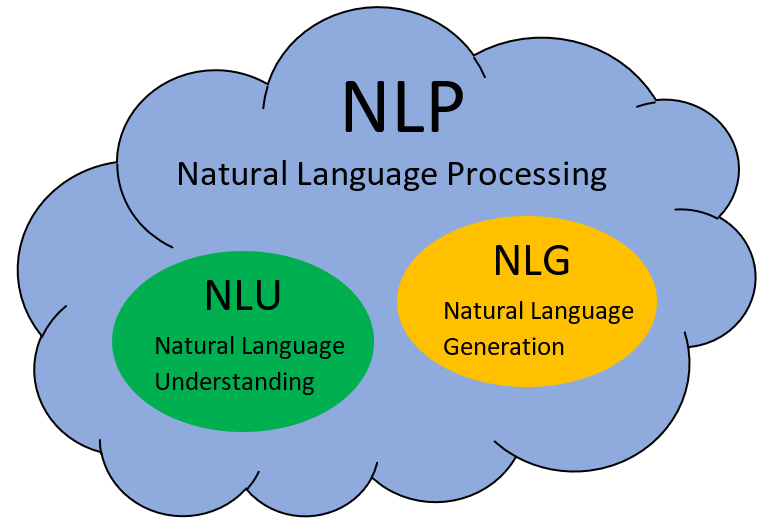
\includegraphics[width=0.5\textwidth]{nlp-nlu-nlg}
    \caption{Grafische voorstelling van NLP en de subdomeinen NLU en NLG \autocite{Sciforce2019}}
\end{figure}

\section{NLP-platformen}
\label{sec:nlp-platformen}

Er zijn tientallen platformen op de markt waarmee chatbots kunnen gebouwd worden. De grootste en meest consistente zijn ontwikkeld en onderhouden door de grote marktspelers zoals Google, Microsoft, IBM, Facebook en Amazon. Een van de zaken die gebouwd kunnen worden met al deze platformen is bijvoorbeeld een chatbot. Ze bieden een gebruiksvriendelijke interface aan waarmee heel eenvoudig chatbots kunnen ontwikkeld worden. Ze hebben ook allemaal hosting mogelijkheden en ingebouwde integraties waarmee zonder moeite de gebouwde bots op andere platformen zoals apps, websites, social media, etc. kunnen gebruikt worden. Binnen vele studies worden hun platformen vaak naar voor geschoven in vergelijking met de kleinere. Daarom zal de vergelijkende studie zich dan ook vooral focussen op platformen die door hen zijn aangeboden omdat zij het kapitaal en de mogelijkheden hebben om te blijven innoveren en hun platformen verder te ontwikkelen. Er zal 1 platform worden onderzocht dat nogal sterk afwijkt van de andere. Dat is omdat dit platform vaak sterk concurreert binnen vergelijkende studies met de andere traditionele. Er zullen enkel platformen worden bekeken die ondersteuning bieden voor de Nederlandse taal, omdat dit een absolute vereiste is voor klanten van In The Pocket die op de belgische markt actief zijn. Het platform van Amazon zal niet worden opgenomen, omdat hun tool geen Nederlands ondersteunt. Verder zullen ook geen betalende platformen worden opgenomen, omdat er voor deze bachelorproef daar geen budget voor is.

\subsection{Dialogflow}
\label{subsec:nlp-platformen-dialogflow}

Dialogflow (vroeger API.ai) is een mens-computer interactie service waarmee verschillende zaken ontwikkeld kunnen worden op basis van natuurlijke taal (Natural Language). Het platform is grotendeels gratis, maar de enterprise edities bieden nog uitgebreidere functies aan. Het is ontwikkeld en onderhouden door Google en maakt gebruik van de infrastructuur en ML-algoritmes van Google. Dialogflow is onderdeel van het Google Cloud Platform (GCP), dat is een platform die heel wat diensten aanbiedt voor applicatie infrastructuur, gegevensbeheer, analyses, machine learning en artificiële intelligentie, beveiliging, etc. Dialogflow is ook geoptimaliseerd voor het gebruik van Google Assistant. Er is ook ondersteuning voorzien voor meer dan 20 talen en er zijn veel intents en entities voorzien die je als ontwikkelaar zomaar out-of-the-box kan gebruiken. Er zijn ook al voorgebouwde chatbots aanwezig voor vaak voorkomende scenario’s die je zomaar kunt gebruiken. Dit platform kan ook geïntegreerd worden in heel erg veel andere diensten. Grote bedrijven zoals Domino’s Pizza, Mercedes, Comcast, Ticketmaster en Giorgio Armani maken onder andere gebruik van Dialogflow voor hun chatbots \autocite{Dialogflow2020}. 

\subsection{IBM Watson}
\label{subsec:nlp-platformen-ibm-watson}

IBM Watson is het NLP-platform van IBM en is net zoals Dialogflow geschikt voor het bouwen van chatbots. Dit platform is deel van IBM cloud, waardoor veel diensten van daar kunnen gebruikt worden. Watson kan voor een beperkt aantal conversaties gratis worden gebruikt. Watson is gebouwd op neurale netwerken, waardoor het heel erg goed kan leren van vorige conversaties. Het ondersteund 13 talen en ook ingebouwde entities. Er zijn ook verschillende integratiemogelijkheden voorzien. IBM Watson staat ook gekend als een platform die heel erg gebruiksvriendelijk is en waarmee in weinig tijd een chatbot kan opgezet worden. Met klanten als The North Face en Chevrolet moeten ze dus zeker niet onderdoen voor de concurrenten \autocite{IBM2020}.


\subsection{LUIS}
\label{subsec:nlp-platformen-luis} 

LUIS is de NLU tool aangeboden door Microsoft en is ook een vaste waarde op de markt. Met LUIS op zich kan geen volledige chatbot worden gebouwd, omdat het enkel NLU diensten aanbiedt en dus enkel dient voor intent classificatie en niet voor het antwoorden naar eindgebruikers toe.  Het kan daarentegen wel makkelijk geïntegreerd worden met het Microsoft Bot Framework, waarin wel de logica zit om complexe dialogen te voeren. LUIS is ook onderdeel van Microsoft Azure, waardoor het ook met deze cloud functies goed kan samenwerken. LUIS maakt gebruik van een speciale active learning technologie waardoor het beter overweg zou kunnen met nieuwe trainingsdata. Er zijn 13 talen ondersteund en ook opnieuw vele ingebouwde intents en entities \autocite{LUIS2020}.

\subsection{Wit.ai}
\label{subsec:nlp-platformen-wit.ai}

Wit.ai is een open-source platform die ontwikkeld is door Facebook. Het is volledig gratis en ondersteund bijna alle talen die er bestaan. Het is een platform door en voor ontwikkelaars en doordat het open source is, is elke interactie gedeeld met de volledige community. Doordat het ontwikkeld is door Facebook, heeft het wel een beperkt aantal integraties (enkel websites, apps en Facebook Messenger) \autocite{Wit2020}.

\subsection{RASA}
\label{subsec:nlp-platformen-rasa}

Het laatste platform die onderzocht wordt is eentje die nogal sterk afwijkt van de andere. Het is verschillend, omdat het ten eerste niet wordt aangeboden door een groot bedrijf zoals Google, Facebook of Microsoft, maar ook omdat het volledig open-source is. Het is ook geen platform die zoals de rest bereikt kan worden via het internet met een user interface. Dit framework moet gedownload worden en dan kan er lokaal een chatbot worden gebouwd. Indien dit platform bereikbaar moet zijn vanop het internet, dan moet de ontwikkelaar daar zelf voor instaan. Het kan wel mits wat configuratie op Google Cloud, Microsoft Azure of Amazon Web Services (AWS) gezet worden. Deze tool vereist heel wat meer technische kennis van ontwikkelaars, maar biedt wel meer mogelijkheden om een chatbot te bouwen die aangepast is aan de noden van een project. Rasa bestaat uit rasa NLU en rasa core.  Rasa NLU staat in voor het classificeren van de intents en het verstaan van berichten en rasa core is een engine om dialogen te voeren. Binnen dit onderzoek zal enkel rasa NLU gebruikt worden. Doordat rasa open-source, kan er als ontwikkelaar zelf worden gekozen welke componenten worden gebruikt. Dit zorgt er voor dat het vrijwel mogelijk is om in elke taal een chatbot met rasa te bouwen. Er zijn ook heel wat componenten beschikbaar om gebruik te maken van voorgemaakte entities en intents. Rasa wijkt sterk af van de andere platformen, maar is zeker interessant om te onderzoeken, omdat het ook vaak in voorgaande studies sterk uit de hoek kwam en omdat het heel sterk op maat geïmplementeerd kan worden \autocite{RASA2020}.

\subsection{Vergelijking van platformen}
\label{subsec:nlp-platformen-vegelijking-platformen}

\begin{center}
    \newcolumntype{P}[1]{>{\hspace{0pt}}p{#1}}
    \begin{longtable}{| P{2.2cm} | p{2.2cm} |  p{2.2cm} | p{2.2cm} | p{2.2cm} | p{2.2cm} |}
        \hline
        \textbf{Naam}                                                  & \textbf{Watson}                                                              & \textbf{LUIS}                           & \textbf{Rasa}                                         & \textbf{Wit.ai}                                 & \textbf{Dialogflow}                                    \\  \hline
        \textbf{Provider}                                              & IBM                                                                     & Microsoft                      & Rasa Technologies Inc.                       & Facebook                               & Google                                        \\  \hline
        \textbf{Gebruiksvriendelijkheid}                               & Hoog                                                                    & Gemiddeld                      & Laag                                         & Gemiddeld                              & Hoog                                          \\  \hline
        \textbf{Prijs initieel gebruik}                                & Gratis                                                                  & Gratis                         & Gratis                                       & Gratis                                 & Gratis                                        \\  \hline
        \textbf{Limieten gratis gebruik}                               & 10000 API calls, 25 intents en 25 entities per maand                    & 10000 API calls per maand      & Onbeperkt                                    & Onbeperkt                              & 180 API calls per minuut                     \\  \hline
        \textbf{Ondersteunde talen}                                    & 13                                                                      & 13                             & Allemaal                                     & 135                                    & 20                                            \\  \hline
        \textbf{Systeem intents}                                       & Nee                                                                     & Ja, grote lijst                & Ja, door specifieke componenten te gebruiken & Nee, Wit.ai bestaat uit enkel entities & Ja, uitgebreide lijst van voorgebouwde agents \\  \hline
        \textbf{Systeem entities}                                      & Ja, 5 in het Nederlands                                                 & Ja, 11 in het Nederlands       & Ja, door specifieke componenten te gebruiken & Ja, 26 in het Nederlands               & Ja, grote lijst voor het Nederlands           \\  \hline
        \textbf{Sentimentanalyse}                                      & Ja                                                                      & Ja                             & Ja                                           & Ja                                     & Ja                                            \\  \hline
        \textbf{Integraties met bestaande diensten}                    & 3 + alles van IBM Cloud                                                 & 11 + alles van Microsoft Azure & 9                                            & 1, Facebook Messenger                  & 18 + Alles van Google Cloud                   \\  \hline
        \textbf{Mogelijkheid tot integratie in eigen websites en apps} & Ja                                                                      & Ja                             & Ja                                           & Ja                                     & Ja                                            \\  \hline
        \textbf{SDK's}                                                 & C\#, Go, Java, Node.js, Python, Ruby, Android, Swift, Unity, Salesforce & C\#, Node.js, Python           & Python                                       & Node.js, Python, Ruby, Go              & C\#, Go, Java, Node.js, PHP, Python, Ruby     \\  \hline
        \textbf{Voorziet API om chatbot te gebruiken en beheren}       & Ja                                                                      & Ja                             & Ja                                           & Ja                                     & Ja                                            \\  \hline
        \textbf{Voorziet hosting}                                      & Ja                                                                      & Ja                             & Nee                                          & Ja                                     & Ja                                            \\  \hline
        \textbf{Spraakondersteuning}                                   & Ja                                                                      & Ja                             & Ja                                           & Ja                                     & Ja                                            \\  \hline
        \textbf{All-in-one platform}                                   & Ja                                                                      & Nee, enkel NLU                 & Ja                                           & Nee, enkel NLU                         & Ja                                            \\  \hline
        \textbf{Default fallback intent}                               & Ja                                                                      & Ja                             & Ja                                           & Nee                                    & Ja   \\ \hline    
        \caption{Vergelijkende tabel van de platformen op basis van de officiële documentatie}                                    
    \end{longtable}
\label{tbl:platformen}
\end{center}

De platformen die hierboven besproken werden, werden ook al vaak in voorgaande studies met elkaar vergeleken. Daaruit bleken telkens andere platformen de bovenhand te nemen. Deze onderzoeken werden ook niet in het Nederlands gedaan, dus een nederlandse vergelijking anno 2020 is dan ook zeker niet overbodig.

Volgens het onderzoek van \textcite{Russis2018} is de tool die IBM aanbiedt om chatbots in de cloud te bouwen veruit de beste op de markt met als dichtste achtervolgers Microsoft (LUIS) en Google (Dialogflow). Dit wordt dan weer betwist door het onderzoek van \textcite{Langen2017}, want zij besluiten dat LUIS (Microsoft) veruit het beste platform is. De eerstvolgende achtervolger is RASA. de resultaten van RASA kwamen vrij dicht in de buurt van die van LUIS. Het grote voordeel van RASA is dat het door de ontwikkelaar helemaal zelf geconfigureerd kan worden, waardoor het beter aangepast kan worden aan een specifieke use case. Het zou dus zeker kunnen dat RASA beter kon presteren dan LUIS mits iets meer configuratie op maat. Dit maakt RASA interessant om verder te onderzoeken.

Volgens het onderzoek van \textcite{Savenkov2017} Is ook IBM Watson de winnaar op het vlak van intent classificatie. Daarnaast zijn Api.ai (nu Dialogflow) en LUIS de eerstvolgende achtervolgers. De verschillen van prestaties tussen die drie zijn relatief klein.

Een ander onderzoek geeft dan weer aan dat Snips.ai de beste NLU heeft met als eerstvolgende achtervolgers Wit.ai en Dialogflow. Snips.ai op zich is een platform dat ook interessante mogelijkheden biedt om verder te onderzoeken, maar dit platform ondersteunt geen Nederlands en is dus niet relevant voor dit onderzoek. Interessant is wel dat Wit.ai en Dialogflow de eerstvolgende achtervolgers zijn \autocite{Coucke2017}.

Uit de verschillende onderzoeken hierboven beschreven kwamen bijna altijd andere platformen naar boven met de beste prestaties voor intent classificatie. Er moet ook rekening gehouden worden met het feit dat deze onderzoeken al enige tijd geleden zijn uitgevoerd en dat de platformen en technologieën binnen AI en ML continu blijven evolueren en dus nu al sterk veranderd zullen zijn. Deze bachelorproef zal een oplossing bieden voor deze onduidelijkheden door een onderzoek anno 2020 uit te voeren.
















